\chapter{Di-$b$-jet Search: Outline and Event Selection}
\label{sec:evt}

In Chapter~\ref{sec:theo} it was shown that many Beyond Standard Model theories
predict new particles decaying to one or two $b$-quarks that could be produced by the LHC.
Chapters~\ref{sec:det},~\ref{sec:obj}~and~\ref{sec:trig}
described the detectors and reconstruction techniques used to observe such an event in the ATLAS detector.
Hence, I have now outlined the motivation and the tools required to perform
a search for resonances decaying to one or two $b$-jets,
an analysis that is called a di-$b$-jet search.

In Chapters~\ref{sec:evt},~\ref{sec:bkg}~and~\ref{sec:lim}
I will describe the di-$b$-jet search analysis using the ATLAS detector.
Each chapter will describe a separate part of the analysis,
the different parts are outlined Section~\ref{sec:evt-outline}.
The di-$b$-jet analysis is performed using three different data-sets,
the data-sets are described in Section~\ref{sec:evt-datasets}.

\section{Analysis Outline}
\label{sec:evt-outline}

The strategy used for the di-$b$-jet analysis
can be split up into broadly three parts.
A brief outline of the parts is given here,
and full detail can be found in the relevant chapter.

\begin{itemize}[leftmargin=*]
\item\textbf{Di-$b$-jet Event Selection:} (\textit{Chapter~\ref{sec:evt}})\\
  The first step is to select events that are consistent with a resonance decaying to one or two $b$-quarks.
  Briefly, we will require two high-momentum jets and consider two $b$-tag categories;
  one where both jets have been $b$-tagged (2 $b$-tag) or where at least one jet has been $b$-tagged ($\geq$ 1 $b$-tag).
  The remainder of the chapter will focus on details of analysis selection;
  Section~\ref{sec:evt-datasets} will describe the data-sets used,
  Section~\ref{sec:evt-s+b} will describe the signal and backgrounds
  considered when defining the selections
  and Section~\ref{sec:evt-sel} will set out
  the details of the event selection used for each of the data-sets.
  \\
\item\textbf{Search Phase:} (\textit{Chapter~\ref{sec:bkg}})\\
  Once events have been selected the next part of the analysis aims to determine if there is
  is a new particle in the selected events; this step is known as the `search phase'.
  For this we will use the \mjj~spectrum, where \mjj~is the invariant mass of the two highest \pT~jets.
  A new particle will appear as a resonance (or `bump') on the smoothly falling
  \mjj~distribution from QCD multi-jet, as illustrated in Figure~\ref{fig:evt-dijet_schem}.
  A fit function is used to model the smoothly falling QCD background and a
  a model-independent search for for resonances is performed using the BumpHunter algorithm.
  Chapter~\ref{sec:bkg} contains a full description of the search phase strategy.
  %including tests of the fitting functions used and the results of the search phase in the data-sets considered.
  \\
  
  \begin{figure}[!hbt]
  \begin{center}
    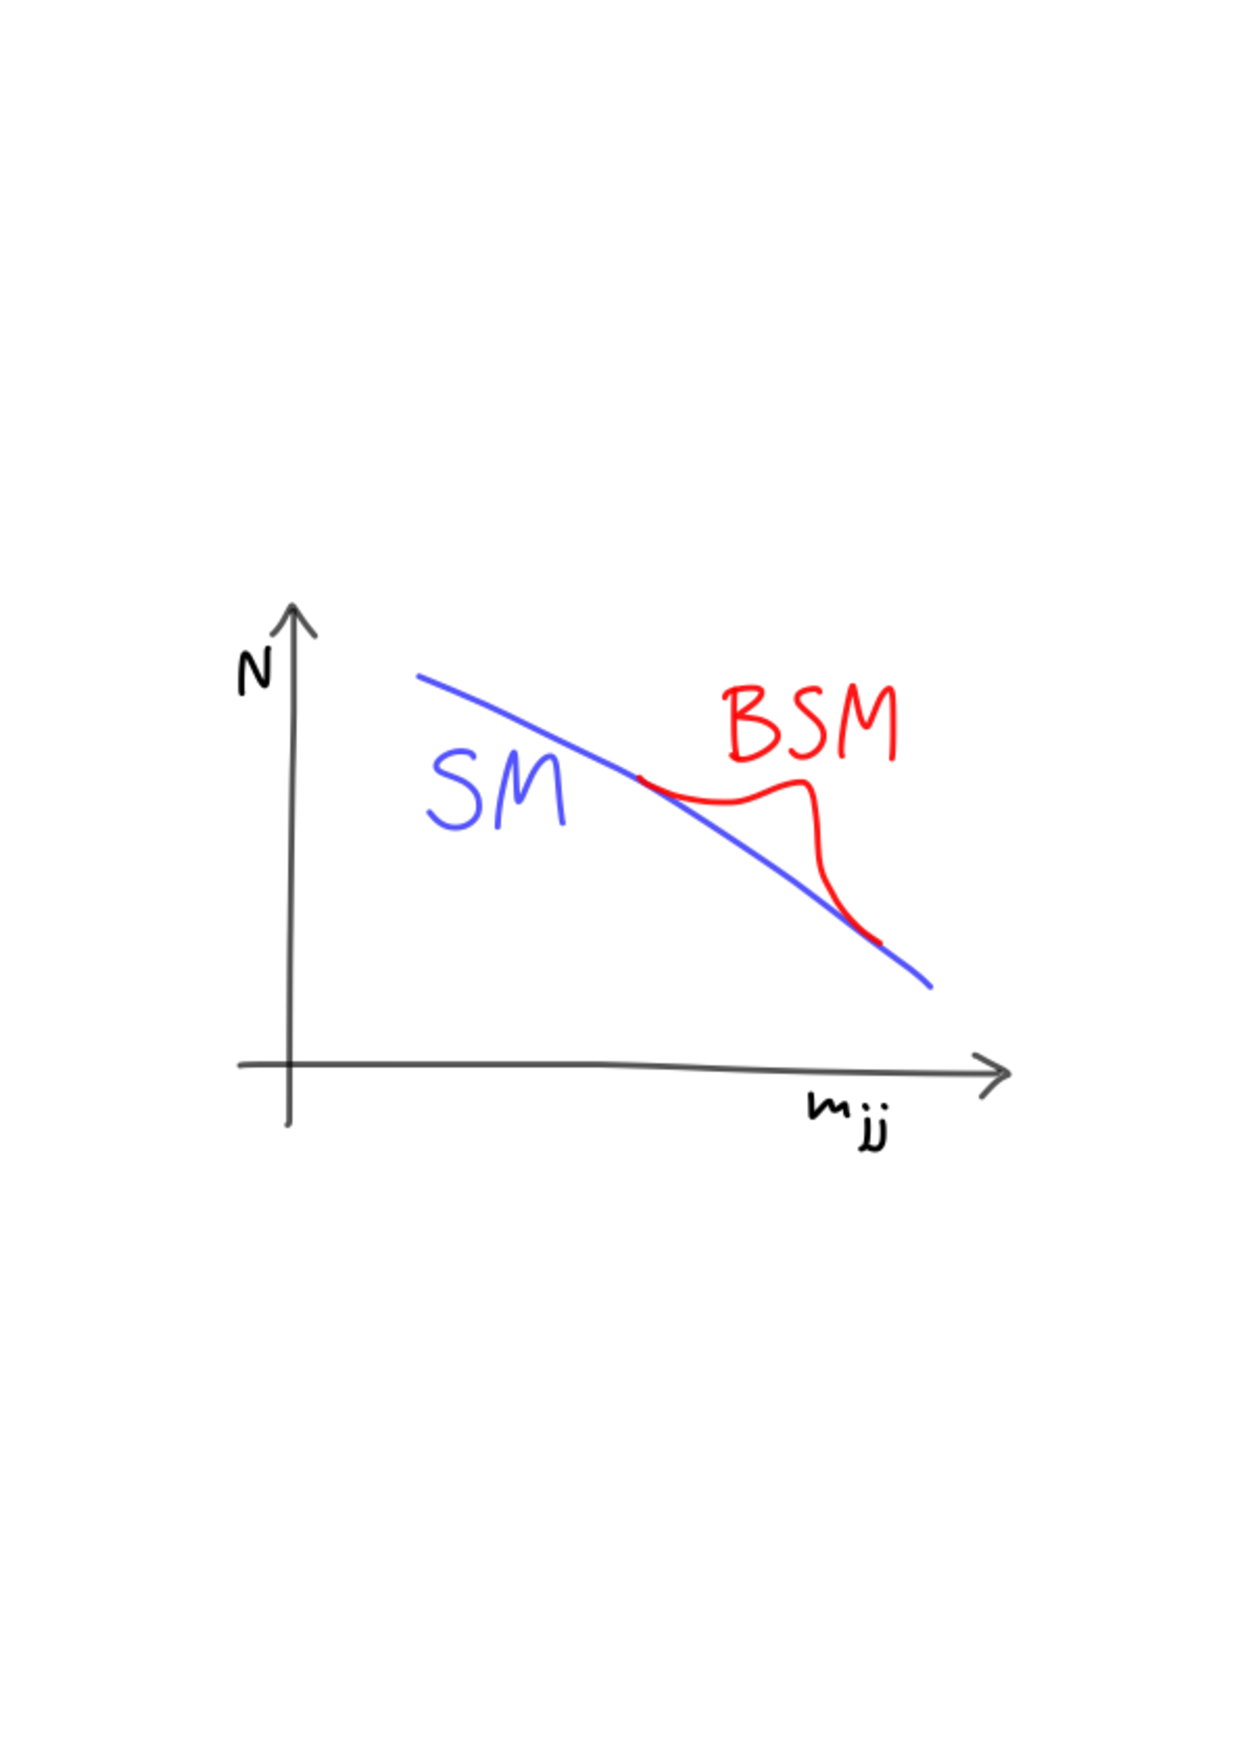
\includegraphics[width=0.5\linewidth, angle=0]{figs/Dibjet/Gen/dijet_schem.pdf}
  \end{center}
  \caption[A cartoon illustrating the use of dijet invariant mass (\mjj) distribution in the search phase of the di-$b$-jet analysis.
    Shown is the expected smoothly falling  distribution of multijet QCD (labelled as SM)
    and a resonance shape due to Beyond Standard Model particle (labelled as BSM)]
          {A cartoon illustrating the use of the dijet invariant mass (\mjj) distribution in the search phase of the di-$b$-jet analysis.
            Shown is the smoothly falling distribution from multijet QCD (SM)
            and a resonance shape caused by a Beyond Standard Model particle (BSM)~\textit{Reference Lene}.}
          \label{fig:evt-dijet_schem}
  \end{figure}
 
\item\textbf{Limit Setting:} (\textit{Chapter~\ref{sec:lim}})\\
  If, in the search phase stage of the analysis, no significant evidence of signal is
  found then it is desirable to quantify what cross-sections can be excluded as a result.
  95\% confidence lower mass limits are set on the two benchmark signals considered.
  The limit-setting methodology, description of systematics considered
  and final limit results in the data sets considered is contained in Chapter~\ref{sec:lim}.

\end{itemize}

\section{List of Data Sets Used}
\label{sec:evt-datasets}

The di-$b$-jet analysis is performed in several iterations
as data is being collected, where each iteration uses a different data-set.
This is done for two reasons;
firstly it is important to know as soon as possible
if there is evidence of a new resonance as
this would affect our strategy moving forward and that of other analyses at ATLAS.
Secondly, this allows us to incrementally
expand, adapt and improve this strategy in each iteration of the analysis.

In this thesis three different data-sets are considered by the di-$b$-jet analysis.
The overall analysis strategy is the same for each data-set,
so the iterations are described together.
However, there are some significant differences in the details;
as such the during the analysis description it will be clearly labelled
which data-set is being referred to.

The data-sets are listed below,
and the trigger and Good Run List (GRL) used in each data-set is described.
The GRL is applied to remove events of low data-quality,
which is typically because an element of the detector was not operating optimally.
For example, data-taking periods where the inner-most layer of the inner detector,
the IBL, was not operating are removed as
this data-taking period had a lower $b$-tagging performance.
All quoted luminosities are given after the GRL has been applied.

\noindent
The data-sets are:

\begin{itemize}[leftmargin=*]
\item\textbf{Summer16+15}: \\
  The \verb|Summer16+15| data-set contains 13 TeV $pp$ collision data collected
  between January 2015 to July 2016 which has an integrated luminosity 13.3~\ifb.
  The trigger used in this data-set, known as \verb|HLT_j380|,
  requires a trigger-level jet with $p_T >$ 380 GeV
  \footnote{\label{foot1} Further details of single-jet triggers is in Section~\ref{sec:trig-jet}.}.
  The analysis on this data-set was made published as a conference note~\cite{dibjet-ichep_conf}. \\
  
\item\textbf{Full16+15\_HighMass}:\\
  The \verb|Full16+15_HighMass| data-set contains 13 TeV $pp$ collision data collected
  between January 2015 to December 2016, which has an integrated luminosity of 36.1~\ifb.
  The trigger used in this data-set, known as \verb|HLT_j380|,
  requires a trigger-level jet with $p_T >$ 380 GeV
  \footnote{Again, see  Section~\ref{sec:trig-jet} for details on single-jet triggers.}.
  The analysis on this data-set has yet to be published.\\
  
\item\textbf{Full16\_LowMass}: \\
  The \verb|Full16_LowMass| data-set contains 13 TeV $pp$ collision data collected
  between January 2016 to December 2016, which has an integrated luminosity of 24.3~\ifb.
  The trigger used in this data-set is known is a double $b$-jet trigger 
  which requires two trigger-level jets with $p_T >$ 150 GeV and $p_T >$ 50 GeV
  where both jets have been $b$-tagged at the trigger level
  \footnote{Further details of $b$-jet triggers and this particular trigger used in this analysis is in Section~\ref{sec:trig-bjet}.}.
  The \verb|Full16_LowMass| uses a $b$-jet trigger as the lower \pT~thresholds allow
  the analysis to probe a lower range of \mjj.
  This analysis did not combine data from 2015 as this used a significantly different $b$-trigger configuration.
  the \verb|Full16_LowMass| uses a $b$-jet trigger aware GRL, which in addition to the normal GRL,
  removed periods of data where the $b$-jet trigger was performing in a sub-optimal way,
  the GRL is described in Section~\ref{sec:trig-grl}.
  As the trigger uses is a double $b$-jet trigger, only the 2 $b$-tag category is considered.
  The analysis on this data-set has yet to be published.

\end{itemize}

\section{Backgrounds and Signal}
\label{sec:evt-s+b}

In the di-$b$-jet analysis selection we consider two
benchmark signal models and one background which will be dominant.
The signal models and dominant background are
used to optimise event selection, so I will describe
the signal and backgrounds considered here.

\begin{itemize}[leftmargin=*]
\item\textbf{Background: QCD Di-jet}: \\
  Section~\ref{sec:theo-qcd} discussed the details of QCD dijet production.
  In particular in Section~\ref{sec:theo-qcd-dijet_features} we noted that the
  relative strength of the strong force compared to other forces
  of the Standard Model means that
  QCD dijet production would dominate other backgrounds in a di-$b$-jet event selection.
  Hence, this will be considered as our only background.
  A description of how the QCD dijet background is modelled in this analysis is described in Chapter~\ref{sec:bkg}.\\

\item\textbf{Signal: $Z'$ Boson}: \\
  The $Z'$ boson is an additional gauge boson that can decay to two $b$-quarks,
  the theoretical $Z'$ models considered are
  described in detail in Section~\ref{sec:theo-bsm_zprime}.
  The $Z'$ boson provides a benchmark model in the 2 $b$-tag category.
  %in the case that both jets have been $b$-tagged.

  In the \verb|Summer16+15| data-set analysis we consider two $Z'$ boson models;
  the first is the Sequential Standard Model (SSM) $Z'$ and the leptophobic $Z'$.
  Monte-Carlo simulation is used to produce \mjj~signal templates;
  this is done using \textsc{Pythia8}~\cite{dibjet-pythia8} with the A14~\cite{dibjet-a14} tune and the NNPDF23LO PDF set~\cite{dibjet-nnpdf}.
  Only decays to $b\bar{b}$ are simulated;
  other decays of the  $Z'$  are ignored such that our
  results are easier to interpret for other signal models decaying to pairs of $b$-quarks.
  Simulated $Z'$ boson templates are produced at mass points of
  1250, 1500, 1750, 2000, 2500, 3000, 4000 and 5000 GeV.
  
  \textbf{LM Fix Full addition}
  In the \verb|Full16+15_HighMass| data-set...
  Similarly the same models are considered in the \verb|Full16+15_LowMass|... \\

\item\textbf{Signal: $b^*$ Quark}: \\
  The $b^*$ quark is the third generation excited quark which results from
  quark compositeness models.
  The dominant decay mode of the  $b^*$ quark is to $bg$.
  The model considered is
  described in detail in Section~\ref{sec:theo-bsm_bstar}.
  The $b^*$ quark provides a benchmark model in the $\geq$1~$b$-tag category.
  %case that at least one of the jets has been $b$-tagged.
    
  
  In the \verb|Summer16+15| and \verb|Full16+15_HighMass|
  data-sets the same $b^*$ model is considered.
  Monte-Carlo simulation is used to produce a $b^*$ \mjj~signal template;
  again \textsc{Pythia8}~\cite{dibjet-pythia8} with the A14~\cite{dibjet-a14} tune and the NNPDF23LO PDF set~\cite{dibjet-nnpdf} is used.
  Decays to $bg$, $b\gamma$, $bZ_0$ and $tW^{-}$ are simulated.
  In the \verb|Full16+15_LowMass| data-set
  only the 2 $b$-tag category is used
  and as such that the $b^*$ model is not considered,
  further details can be found in Section~\ref{sec:evt-sel-btag}.
  Simulated $b^*$ quark templates are produced at mass points of
  1250, 1500, 1750, 2000, 2500, 3000, 4000 and 5000 GeV.
\end{itemize}

\section{Event Selection}
\label{sec:evt-sel}

The overall aim when designing the di-$b$-jet analysis event selection
is two-fold.
Firstly, events are selected to
maximise sensitivity to signal;
which we approximate in terms of $S$/$\sqrt{B}$,
where $S$ is the number of benchmark signal events and $B$ is the number of background events.
Secondly, we need to maintain the smoothly falling nature of the background
as this is the underlying assumption of the background estimation strategy,
which will be described in Chapter~\ref{sec:bkg}.

The di-$b$-jet event selection is split up into three sections each described separately.
Firstly we select a pair of jets to be considered (Section~\ref{sec:evt-sel-jets}),
then we apply a set of event-level kinematic cuts using the selected jets (Section~\ref{sec:evt-sel-event})
and finally we apply $b$-tagging to the jets (Section~\ref{sec:evt-sel-btag}).
In section~\ref{sec:evt-sel-acc} the total signal acceptance of the
event selection is evaluated.

The event selection is slightly different for each of the data-sets considered,
these differences will be noted and discussed in the text.

\subsection{Jet Selection}
\label{sec:evt-sel-jets}

Jets are reconstructed using the anti-$k_T$ algorithm with $R=0.4$
and calibrated using the EM+JES scheme;
a full description of jets used in this analysis is in Section~\ref{sec:obj-jets}.

At least two jets are required in an event.
The two highest \pT~jets, referred to as the leading and subleading jet,
are the jets used throughout this analysis.
To reduce the number of fake jets from sources such as calorimeter noise
both jets are required to pass \textit{loose} jet cleaning cuts
based on the properties and distributions of the energy deposits in the calorimeter associated to the jet;
details can be found in~\cite{evt-jet_cleaning}.

Cuts are applied to the leading and subleading jet-\pT~such that events are on the trigger plateau;
the kinematic region where all events passing the offline jet-\pT~selection
would also pass the online jet-\pT~requirements of the trigger
\footnote{Online refers to reconstructed objects used in the trigger decision
  whilst offline refers to objects reconstructed after events have passed the trigger at the data-processing level,
  from the definition in Section~\ref{sec:trig-bjet_eff}.}.

For the \verb|Summer16+15| data-set; it is required that the leading jet has \pT~$>$ 430 GeV to be on the trigger plateau of \verb|HLT_j380|.
This cut is derived by comparing the leading jet-\pT~distributions of jets that pass the trigger, \verb|HLT_j380|,
relative to a benchmark trigger with a lower jet-\pT~threshold, \verb|L1_J75|.
Figure~\ref{fig:evt-jet_pt} shows this comparison in one run of data where \verb|L1_J75| was un-prescaled
\footnote{Un-prescaled means that the trigger accepts every event passing the trigger criteria};
in the ratio plot it is shown that for leading jet-\pT~$>$ 430 GeV events are on the trigger plateau.
The subleading jet is required to have jet-\pT~$>$ 60 GeV,
to avoid contamination from pile-up jets.
Both jets  are required to have $|\eta| <$ 2.4
such that the jets lie within the volume of the ATLAS pixel detector,
which is essential for optimal $b$-tagging performance.

\begin{figure}[!ht]
  \begin{center}
    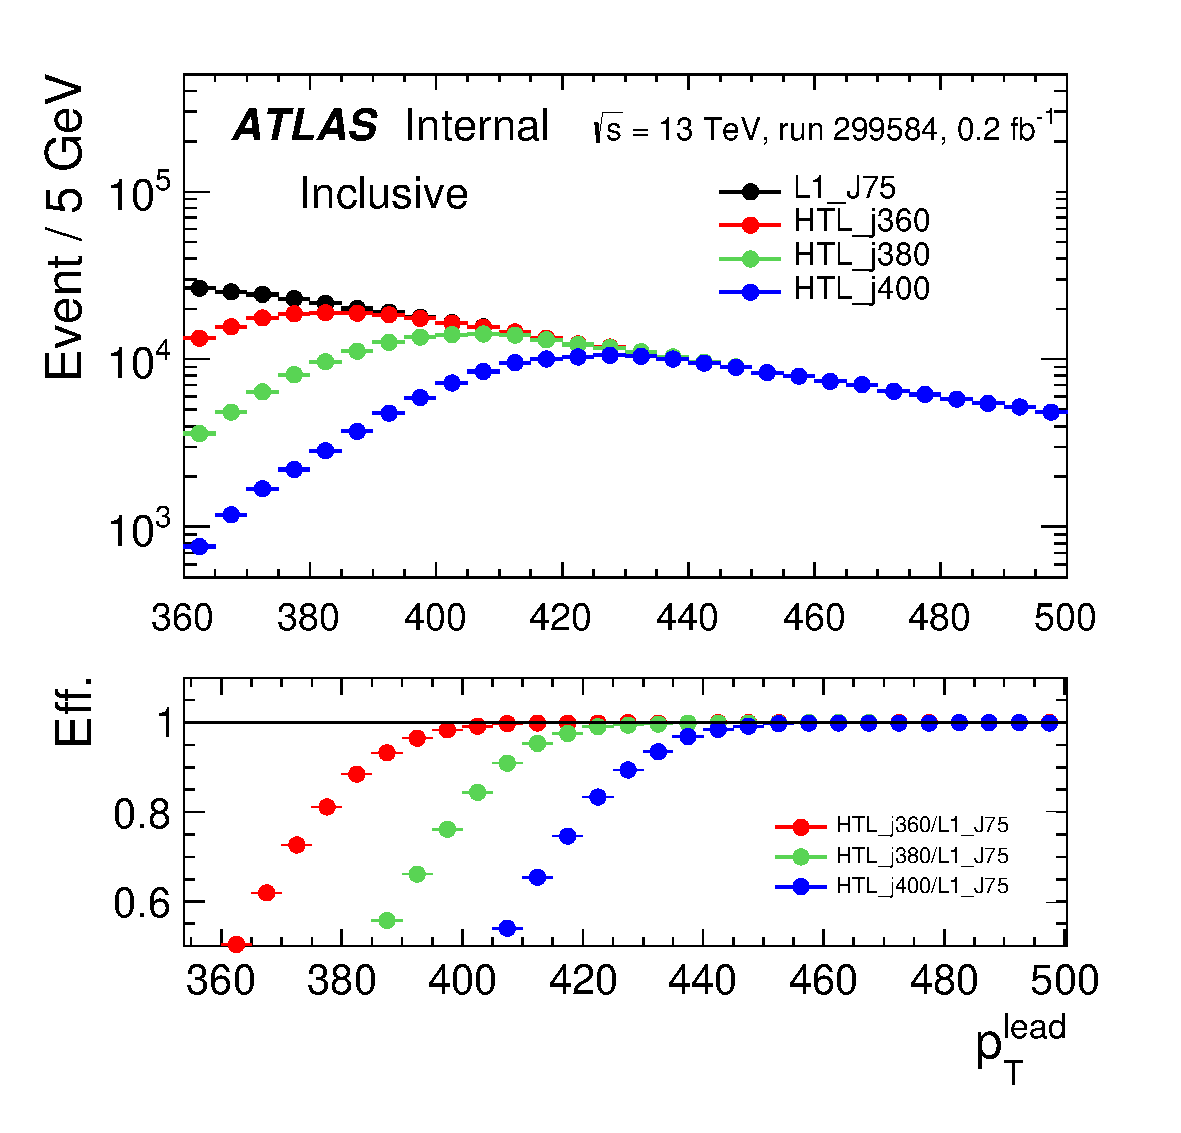
\includegraphics[width=0.8\linewidth, angle=0]{figs/Dibjet/ICHEP/evt-jet_pt.pdf}
  \end{center}
\caption[The comparisons of the leading jet-\pT~using unprescaled L1\_J75 trigger (black dots) to the HLT\_J360 trigger (red dots),
  HLT\_J380 trigger (green dots) and HLT\_J400 trigger (blue dots) in one run of 2016 data.
  The ratio with respect to L1\_J75 is shown in the lower panel.]
        {The comparisons of the leading jet-\pT~using an unprescaled L1\_J75 trigger (black dots) to the HLT\_J360 trigger (red dots),
          HLT\_J380 trigger (green dots) and HLT\_J400 trigger (blue dots) in one run of 2016 data.
          The ratio with respect to L1\_J75 is shown in the lower panel~\cite{dibjet-ichep_conf}.}
  \label{fig:evt-jet_pt}
\end{figure}

\subsection{Event Level Cuts}
\label{sec:evt-sel-event}

Using the two selected jets; there are a set of event-level requirements
split into three parts.
Firstly, events are required to have good reconstruction quality;
specifically the primary vertex \textbf{LM Fix: Primary Vertex selection to be added to tracking}
must have at least two tracks associated with it
and events with problematic reconstruction in the Tile calorimeter, LAr calorimeter or SCT are rejected.
\textbf{LM Fix, not sure what these are}

\noindent
Secondly, we increase sensitivity to signal using the 
variable $y^*$, defined as
\begin{equation}
  y^* = \frac{(y_1-y_2)}{2}
\end{equation}
where $y_1$ and $y_2$ are the rapidities of the leading and subleading jet respectively.
As discussed in Section~\ref{sec:theo-qcd-dijet_features}, QCD dijet production can occur through $t$-channel processes leading to more background events at large values of $|y^*|$,
whilst signal production occurs only through $s$-channel processes so will have no dependence on $y^*$.
Therefore, requiring $|y^*|$ below some threshold value will lead to an increased $S/\sqrt{B}$.

In the \verb|Summer16+15| data-set we require $|y^*| <$ 0.6.
This value has been shown to maximise $S/\sqrt{B}$ when no $b$-tagging is applied
at previous inclusive dijet searches at ATLAS~\cite{dijet-mori16_paper}
\footnote{Inclusive dijet analysis means a dijet analysis where no $b$-tagging is applied}.
The effect of $b$-tagging on the optimal value of this cut is likely to be small,
as $t$-channel processes still dominate the background.

Thirdly, the invariant mass of the two leading jets, \mjj, is required to above a threshold value.
This cut ensures that there is no kinematic bias on the \mjj~distribution
from the trigger or jet-\pT~requirements described in Section~\ref{sec:evt-sel-jets}.
In addition, it is also required that the background is smooth in the \mjj~region chosen
such that it can be described using our background modelling strategy.

In the \verb|Summer16+15| data-set we require \mjj~\gt~1378 GeV;
which ensures the two conditions listed above are met.
Firstly, Figure~\ref{fig:evt-mjj} shows the comparison of \mjj~distributions for events
that pass the analysis jet-\pT~requirements and  trigger, \verb|HLT_j380|, compared to events that pass a reference trigger, \verb|L1_J75|
in one run of data where \verb|L1_J75| was un-prescaled.
The ratio plot demonstrates that for \mjj~\gt~1100 GeV there is no kinematic bias from the trigger or jet-\pT~cuts.
%therefore we conclude that for \mjj~\gt~1378 GeV there is also no kinematic bias.
Secondly, it has been shown using simulated events that
\mjj~\gt~1378 GeV is required such that the \mjj~distribution from QCD dijet production
can be described by our background modelling strategy;
this study is presented in Section~\ref{sec:bkg-summer_range}.
Hence, \mjj~\gt~1378 GeV is the loosest cut that meets both of the conditions.

\begin{figure}[!ht]
  \begin{center}
    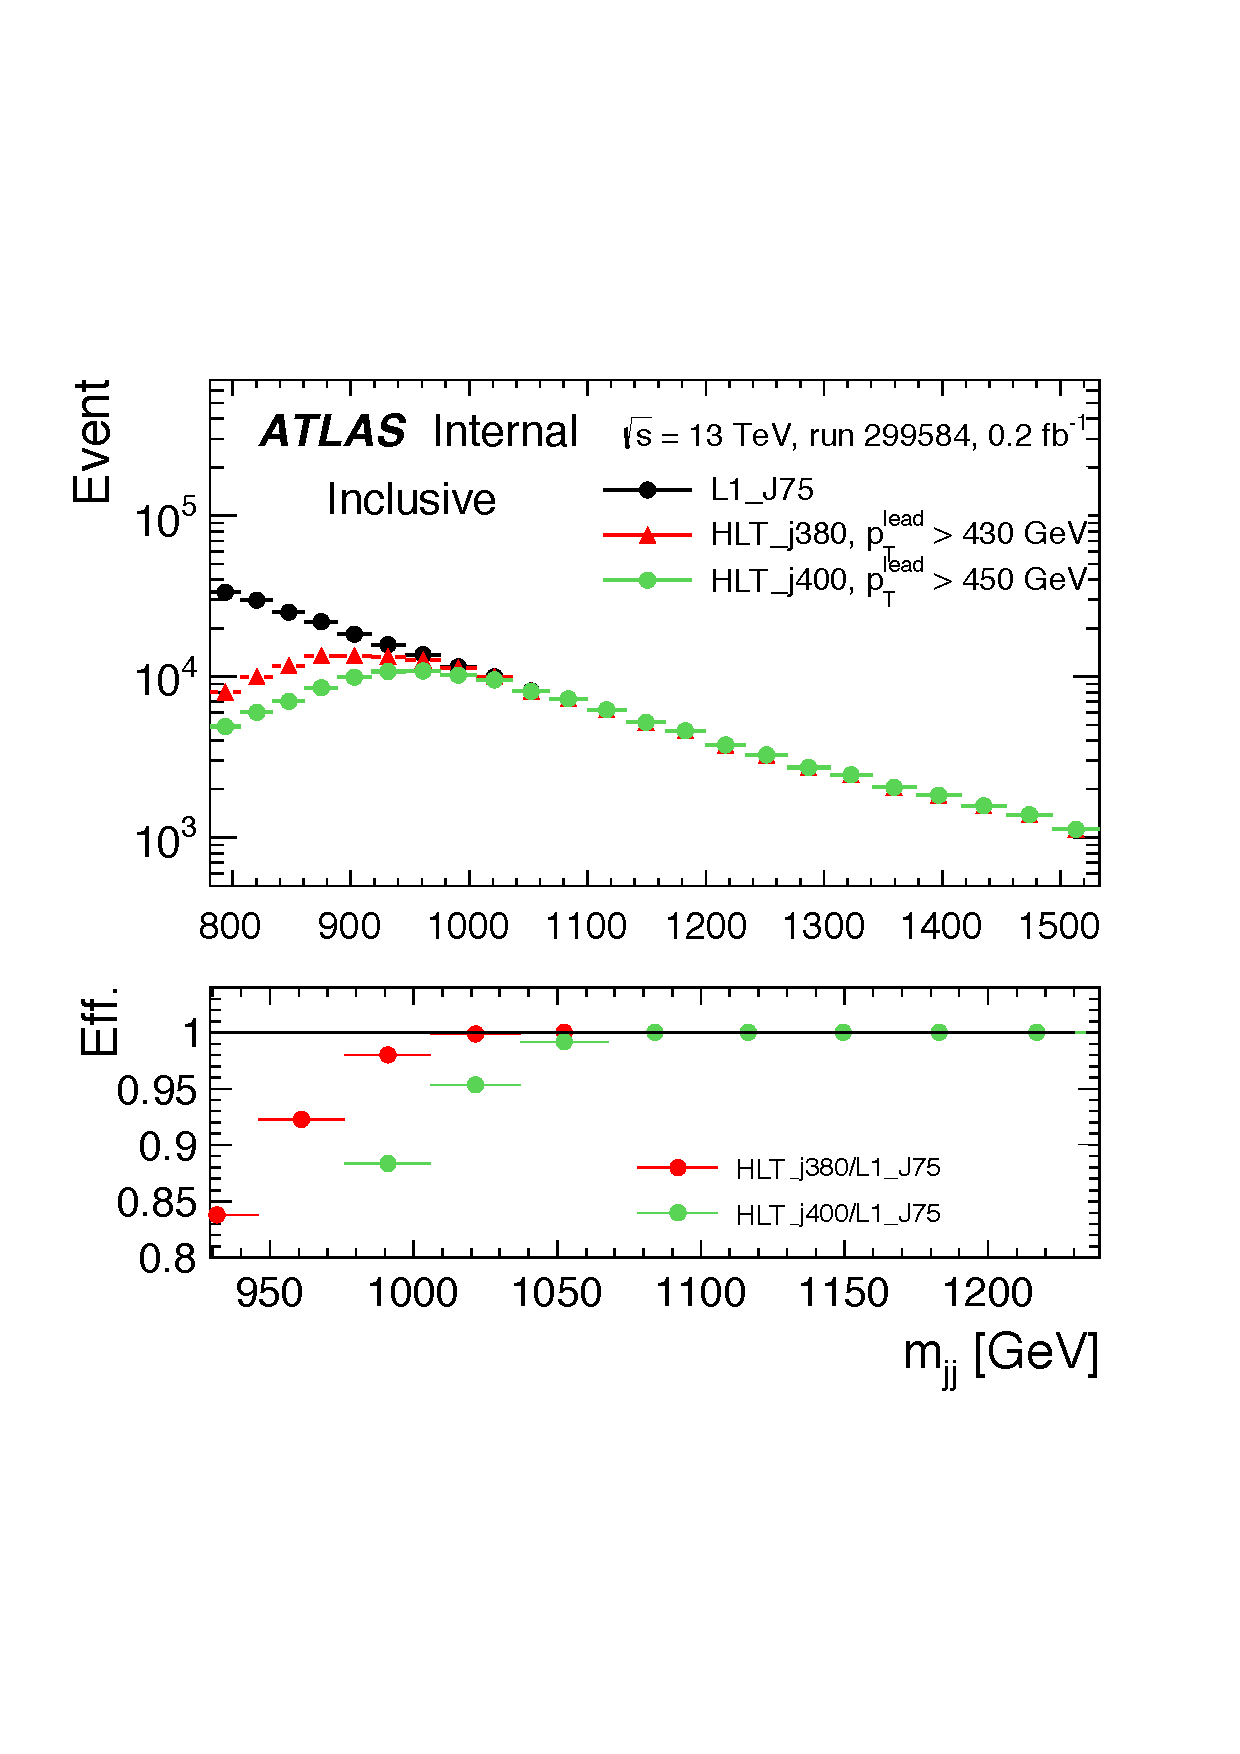
\includegraphics[width=0.8\linewidth, angle=0]{figs/Dibjet/ICHEP/evt-mjj.pdf}
  \end{center}
  \caption[The comparisons of the \mjj~distribution of events that pass an unprescaled L1\_J75 trigger (black dots) to the
    events that pass the HLT\_J380 trigger with leading jet-\pT~\gt~430 GeV (red dots) and 
    the HLT\_J400 trigger with a leading jet-\pT~\gt~450 GeV (green dots) in one run of 2016 data.
    The ratio with respect to L1\_J75 is shown in the lower panel.]
        {The comparisons of the \mjj~distribution of events that pass an unprescaled L1\_J75 trigger (black dots) to the
    events that pass the HLT\_J380 trigger with leading jet-\pT~\gt~430 GeV (red dots) and 
    the HLT\_J400 trigger with a leading jet-\pT~\gt~450 GeV (green dots) in one run of 2016 data.
    The ratio with respect to L1\_J75 is shown in the lower panel~\cite{dibjet-ichep_conf}.}
  \label{fig:evt-mjj}
\end{figure}

\subsection{$b$-Tagging}
\label{sec:evt-sel-btag}

The selection of $b$-jets, known as $b$-tagging,
and forms an essential technique in the di-$b$-jet event selection.
A detailed description of $b$-tagging is found in Section~\ref{sec:obj-bjets}.
$b$-tagging is performed using a multi-variate algorithm known as MV2c10 which has been described in~\ref{sec:obj-bjets_MV2}.

Two $b$-tagging categories are used for the two different types of signal model considered.
The 2 $b$-tag category requires that the both jets are $b$-tagged,
and is used to search for resonances decaying to 2 $b$-quarks such as the $Z'$ boson.
The $\geq 1$ $b$-tag category requires that at least one jet is tagged,
and is used to search for resonances decaying to 1 $b$-quark and a quark/gluon such as the $b^*$ quark.
The exclusive 1 $b$-tag category was also considered but was found to be less sensitive to the $b^*$ model.

In the \verb|Summer16+15| and \verb|Full16+15_HighMass| data-sets
$b$-tagging is performed using the fixed cut 85\% operating point of the MV2c10 algorithm
\footnote{Details on the operating points of MV2c10 are found in~\ref{sec:obj-bjets_MV2}}.
This operating point was chosen to maximise $S/\sqrt{B}$ for a range of signal mass points in the 2 $b$-tag category.

Below are details of the $b$-tagging optimisation study for the \verb|Full16+15_HighMass| data-set are shown,
the results also validate the choice of $b$-tagging operating point in the \verb|Summer16+15| data-set.
The number of background events, $B$, is estimated in
a narrow mass window around
each mass point considered using a
18.9~\ifb~subset of data for the 2 $b$-tag category.
The number of signal events, $S$, is estimated
in the same narrow mass windows using 
the simulated SSM $Z'$-boson signal template
described in Section~\ref{sec:evt-s+b} scaled to 18.9~\ifb.
The full \verb|Full16+15_HighMass| event selection has been applied.
Table~\ref{tab:evt-btag_hm} summarises the $S/\sqrt{B}$ for each operating point;
the 85\% operating point is selected as it performs well across the full range of mass points considered.
The conclusions of this study are luminosity independent
as $S/\sqrt{B} \propto 1/\sqrt{L}$ such that the relative sensitivity
between operating points will be the same for all luminosities.

\begin{table}[ht]
\begin{center}
\begin{tabular}{|c||c|c|c|}
  \hline
  Mass of $Z'$ boson [GeV]        &  1500  &   2000  &  2500  \\
  \hline
  Mass window [GeV]               & 1378-1573       &  1785-2114   &  2267-2659 \\
  \hline
  $S/\sqrt{B}$ for 85\% OP        &  2.02           &  0.72        &  0.21          \\
  $S/\sqrt{B}$ for 77\% OP        &  2.12           &  0.64        &  0.17          \\
  $S/\sqrt{B}$ for 70\% OP        &  1.73           &  0.47        &  0.12          \\
  $S/\sqrt{B}$ for 60\% OP        &  0.96           &  0.21        &  0.07          \\ \hline
\end{tabular}
\caption{The estimated $S/\sqrt{B}$ at 18.9~\ifb~for 4 different MV2c10 operating points (OP).
  $S$ is estimated using a SSM $Z'$-boson and $B$ is estimated using a 18.9~\ifb~subset of 2 $b$-tag category data.
  The \textit{Full16+15\_HighMass} data-set event selection has been applied.
  Three different mass points are considered and the mass windows used
  to estimate $S$ and $B$ for each mass point are shown in the table~\cite{dibjet-ichep_int}.}
\label{tab:evt-btag_hm}
\end{center}
\end{table}

The background flavour composition is studied to better understand the effect of the flavour composition in this analysis.
The dijet flavour composition is defined as the truth flavour of both of the jets used in the di-$b$-jet analysis,
using the definition of truth flavour from Section~\ref{sec:obj-bjets_label}.
Figure~\ref{fig:evt-summer_flavcomp} shows the dijet flavour composition of the simulated QCD dijet background in
the case where no $b$-tagging has been applied (inclusive) and in the $\geq1$ and 2 $b$-tag categories.
For this figure the \verb|Summer16+15| data-set event selection has been applied,
although the distributions are very similar for the \verb|Full16+15_HighMass| data-set
as the same $b$-tagging operating point has been chosen.

\begin{figure}[!ht]
  \begin{center}
    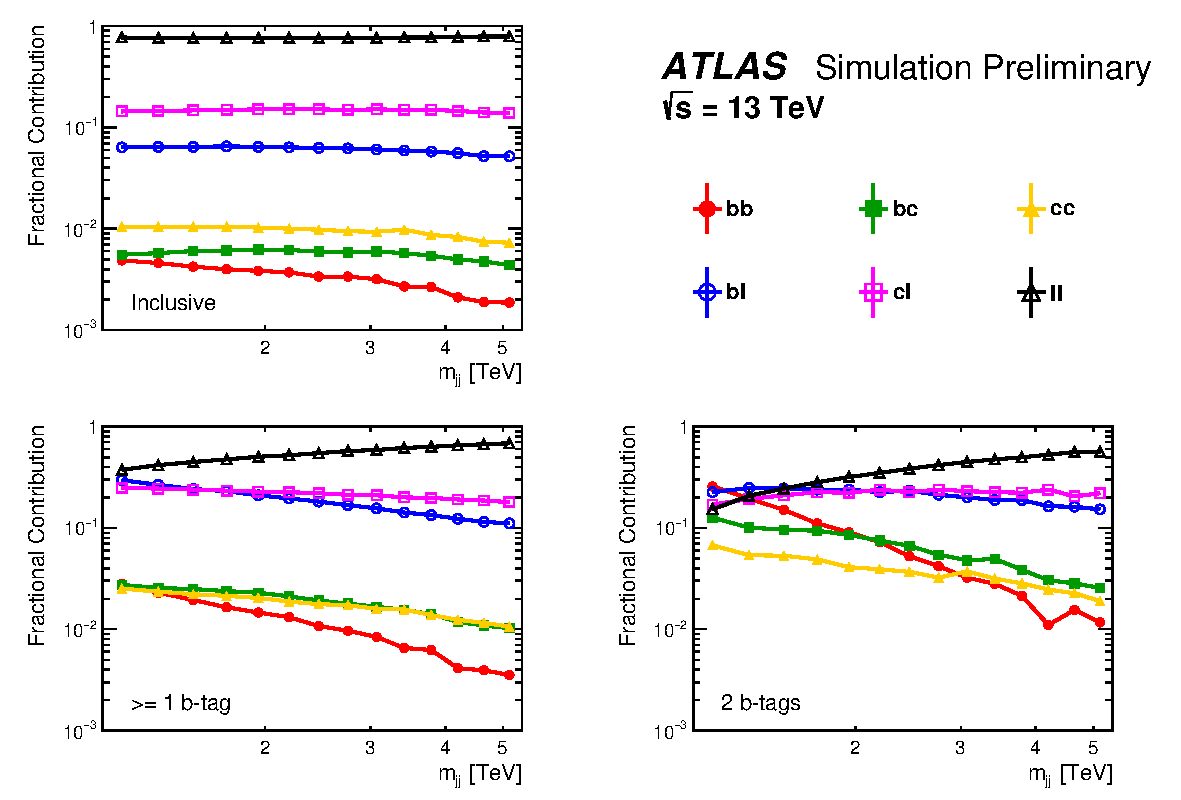
\includegraphics[width=0.99\linewidth, angle=0]{figs/Dibjet/ICHEP/evt-summer_flavcomp.pdf}
  \end{center}
  \caption{The dijet flavour composition of the simulated dijet background as a function of dijet mass,
    shown without applying $b$-tagging (inclusive) and for $\geq1$ $b$-tag and 2 $b$-tag categories.
    In the legend b, c and l refere to a truth matched $b$-jet, $c$-jet and light jet respectively.
    The \textit{Summer16+15} dataset event selection has been applied.}
  \label{fig:evt-summer_flavcomp}
\end{figure}

There are a few features that can be noted in this figure.
Firstly, the figure shows that the flavour fraction of the background before $b$-tagging is dominated by light-jets
for the reasons outlined in~Section~\ref{sec:theo-qcd-dijet_features}.
As the background is dominated by light-jets the application
of $b$-tagging can sigificantly increase background rejection
and thus increase sensitivity to signal models that decay to $b$-quarks.
This motivates the use of $b$-tagging in the analysis.

Secondly, even after the application of $b$-tagging the largest contribution to the background is from light jets,
except for in a small region at low mass in the 2 $b$-tag category.
This shows that the sensitivity of the analysis is limited by the
$b$-tagging performance at high jet-\pT.

Finally, in all three cases the dijet flavour fractions are smooth, which is evidence that
there are no sudden changes in $b$-tagging efficiency of the background that could introduce
a non-smooth feature in the background invariant mass spectra.

\subsection{Event Selection Summary}
\label{sec:evt-sel-acc}

The  key components
of the di-$b$-jet event selection
for each of the data-sets considered
as descibed in this Chapter
is listed Table~\ref{tab:evt}.

\begin{table}[!htb]
  \begin{tabular}{|c||c|c|c|}
    \hline
\thead{Cut}              &  \thead{Summer16+15} & \thead{Full16+15\_HighMass} & \thead{Full16+15\_LowMass} \\
\hline
%Trigger          & HLT\_380 & HLT\_380 & \makecell{ HLT\_j150\_bmv2c2060\_split\\\_j50\_bmv2c2060\_split} \\
Trigger                & Single-jet       & Single-jet    & Double $b$-jet (60\% OP) \\
Online LJ~\pT          & \gt~380 GeV      & \gt~380 GeV   & \gt~150 GeV  \\
Online SLJ~\pT         & -                & -             & \gt~50 GeV \\
\hline
Leading Jet-\pT    &  \gt~430 GeV & \gt~430 GeV &  \gt~200~GeV\\
Subleading Jet-\pT &  \gt~60 GeV & \gt~80 GeV  &  \gt~80~GeV\\
Jet-$|\eta|$   & $<$ 2.4 & $<$ 2.0 & $<$ 2.0 \\
\hline
$m_{jj}$  & \gt~1378 GeV & \makecell{\gt~1200 GeV (2 $b$-tag)\\ \gt~1341 GeV ($\geq1$ $b$-tag)} & \gt~500 GeV \\
$|y^*|$  & $<$ 0.6 & $<$ 0.8 & $<$ 0.6  \\
\hline
$b$-Tagging OP & 85\% & 85\% & 70\%\\
$b$-Tag Categories & 2 and $\geq$1 & 2 and $\geq$1 & 2 \\
\hline
\end{tabular}
\centering
\caption{A summary of the key event selections applied in the di-$b$-jet analysis for each of the data-sets considered.
For full details refer to the text.}
\label{tab:evt}
\end{table}

To better visualise events that pass the event selection,
Figure~\ref{fig:evt-vp1} show events displays for high~\mjj~events that pass
the $\geq$1 and 2 $b$-tag $b$-tag event selection respectively.
The figure was made using the VP1 event display package~\ref{evt-vp1}.
These events are included in and pass both the \verb|Summer16+15| and \verb|Full16+15_HighMass| data-set event selection.

\begin{figure}[!ht]
  \begin{center}
    \captionsetup[subfigure]{aboveskip=0pt,justification=centering}
    \subcaptionbox{2 $b$-tag\vspace{5mm}}      {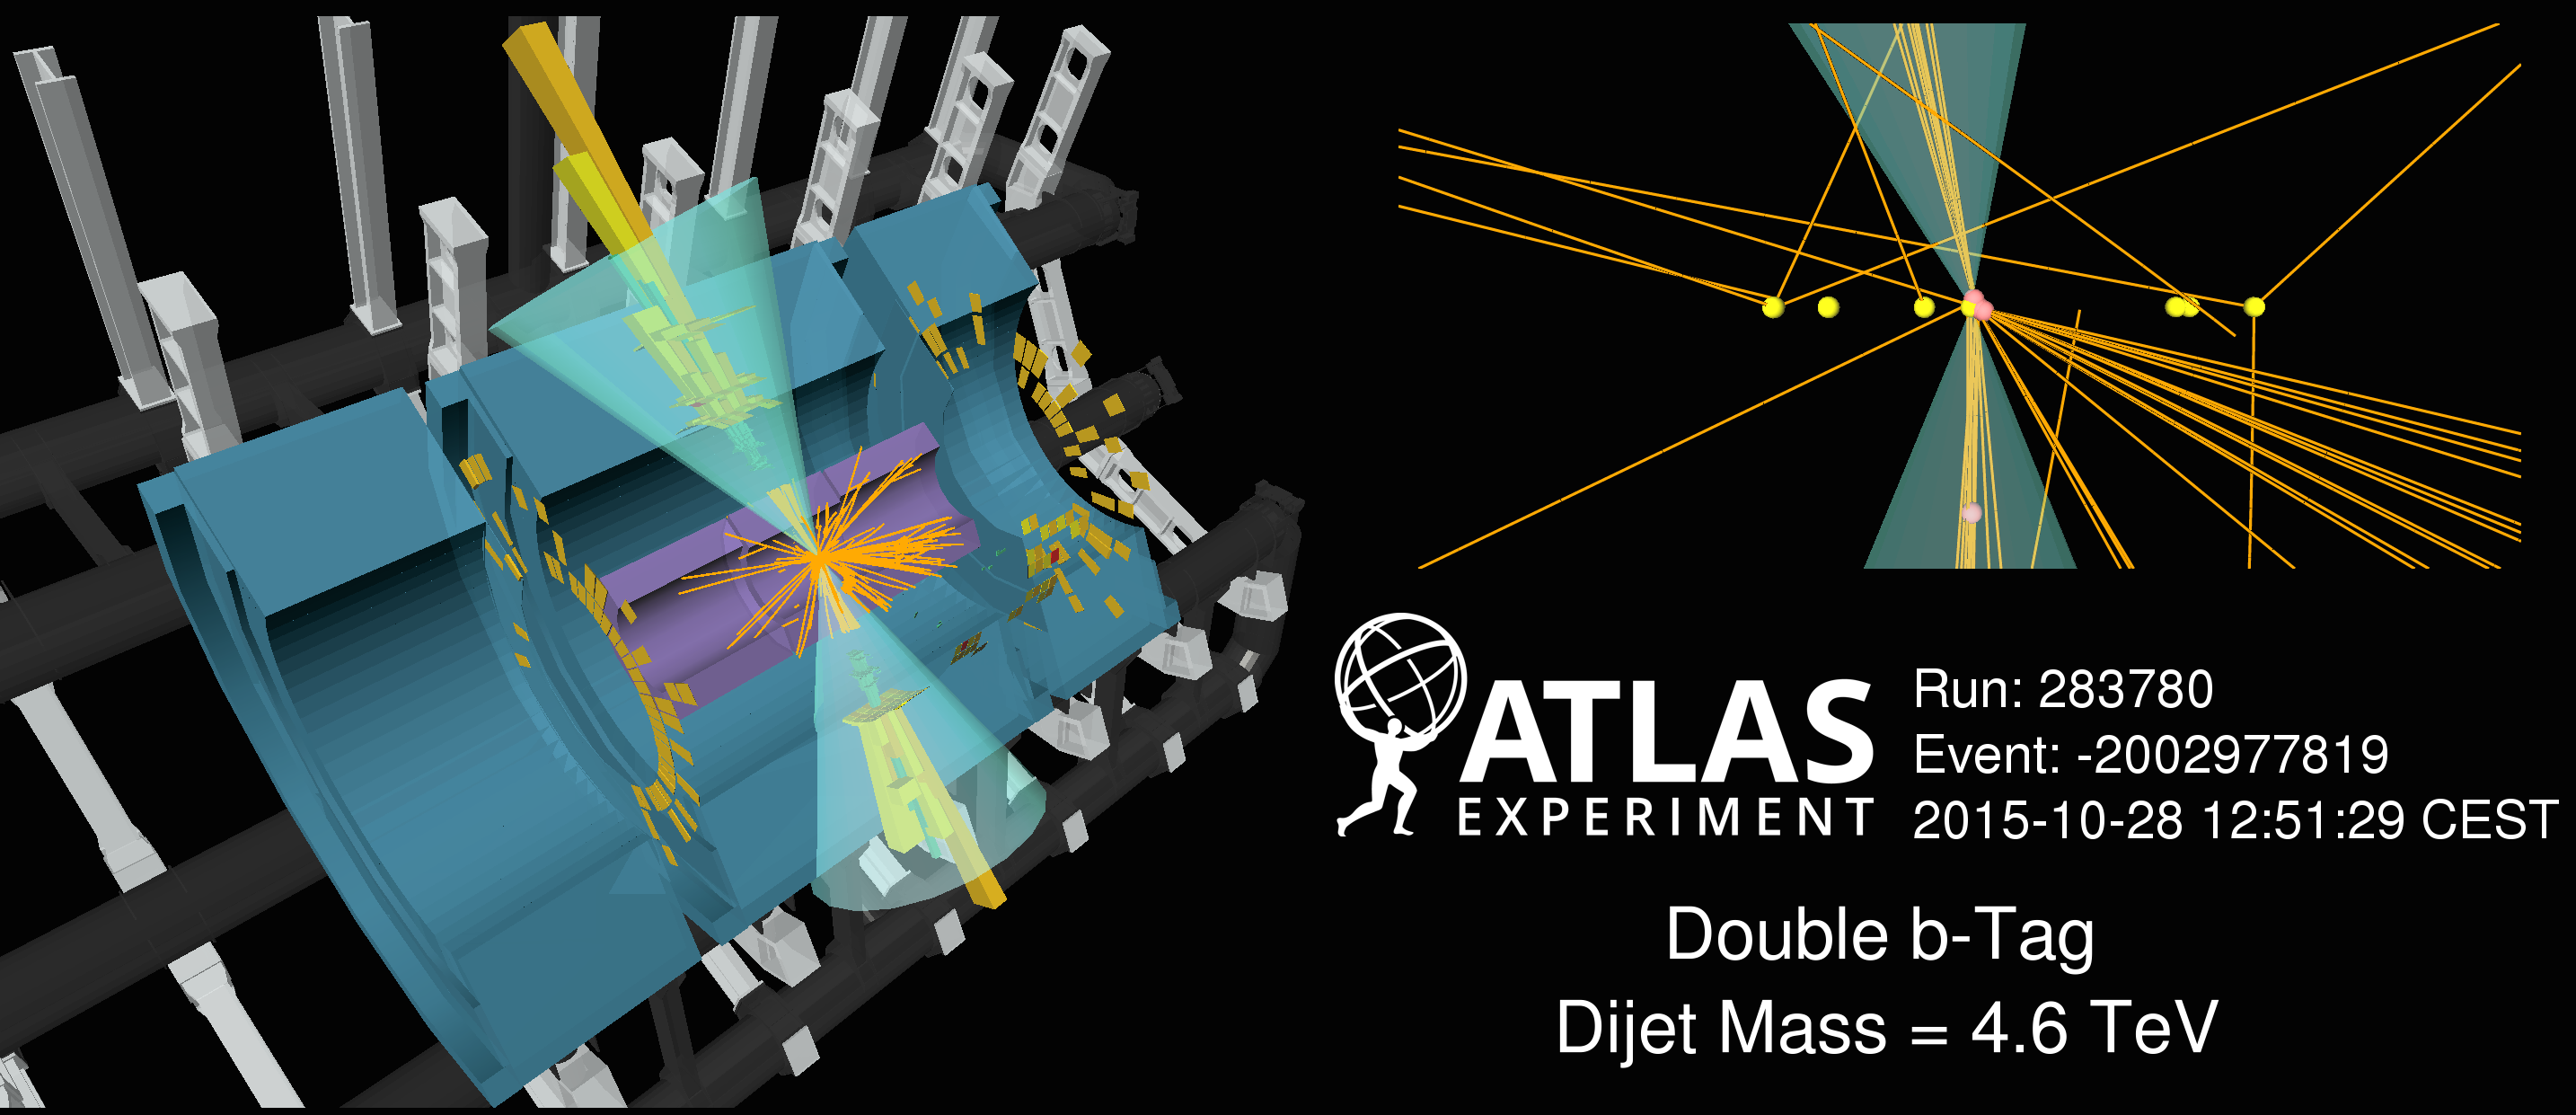
\includegraphics[width=0.95\linewidth, angle=0]{figs/Dibjet/Gen/evt-vp1_bb.png}}\\
   \subcaptionbox{$\geq$1 $b$-tag}{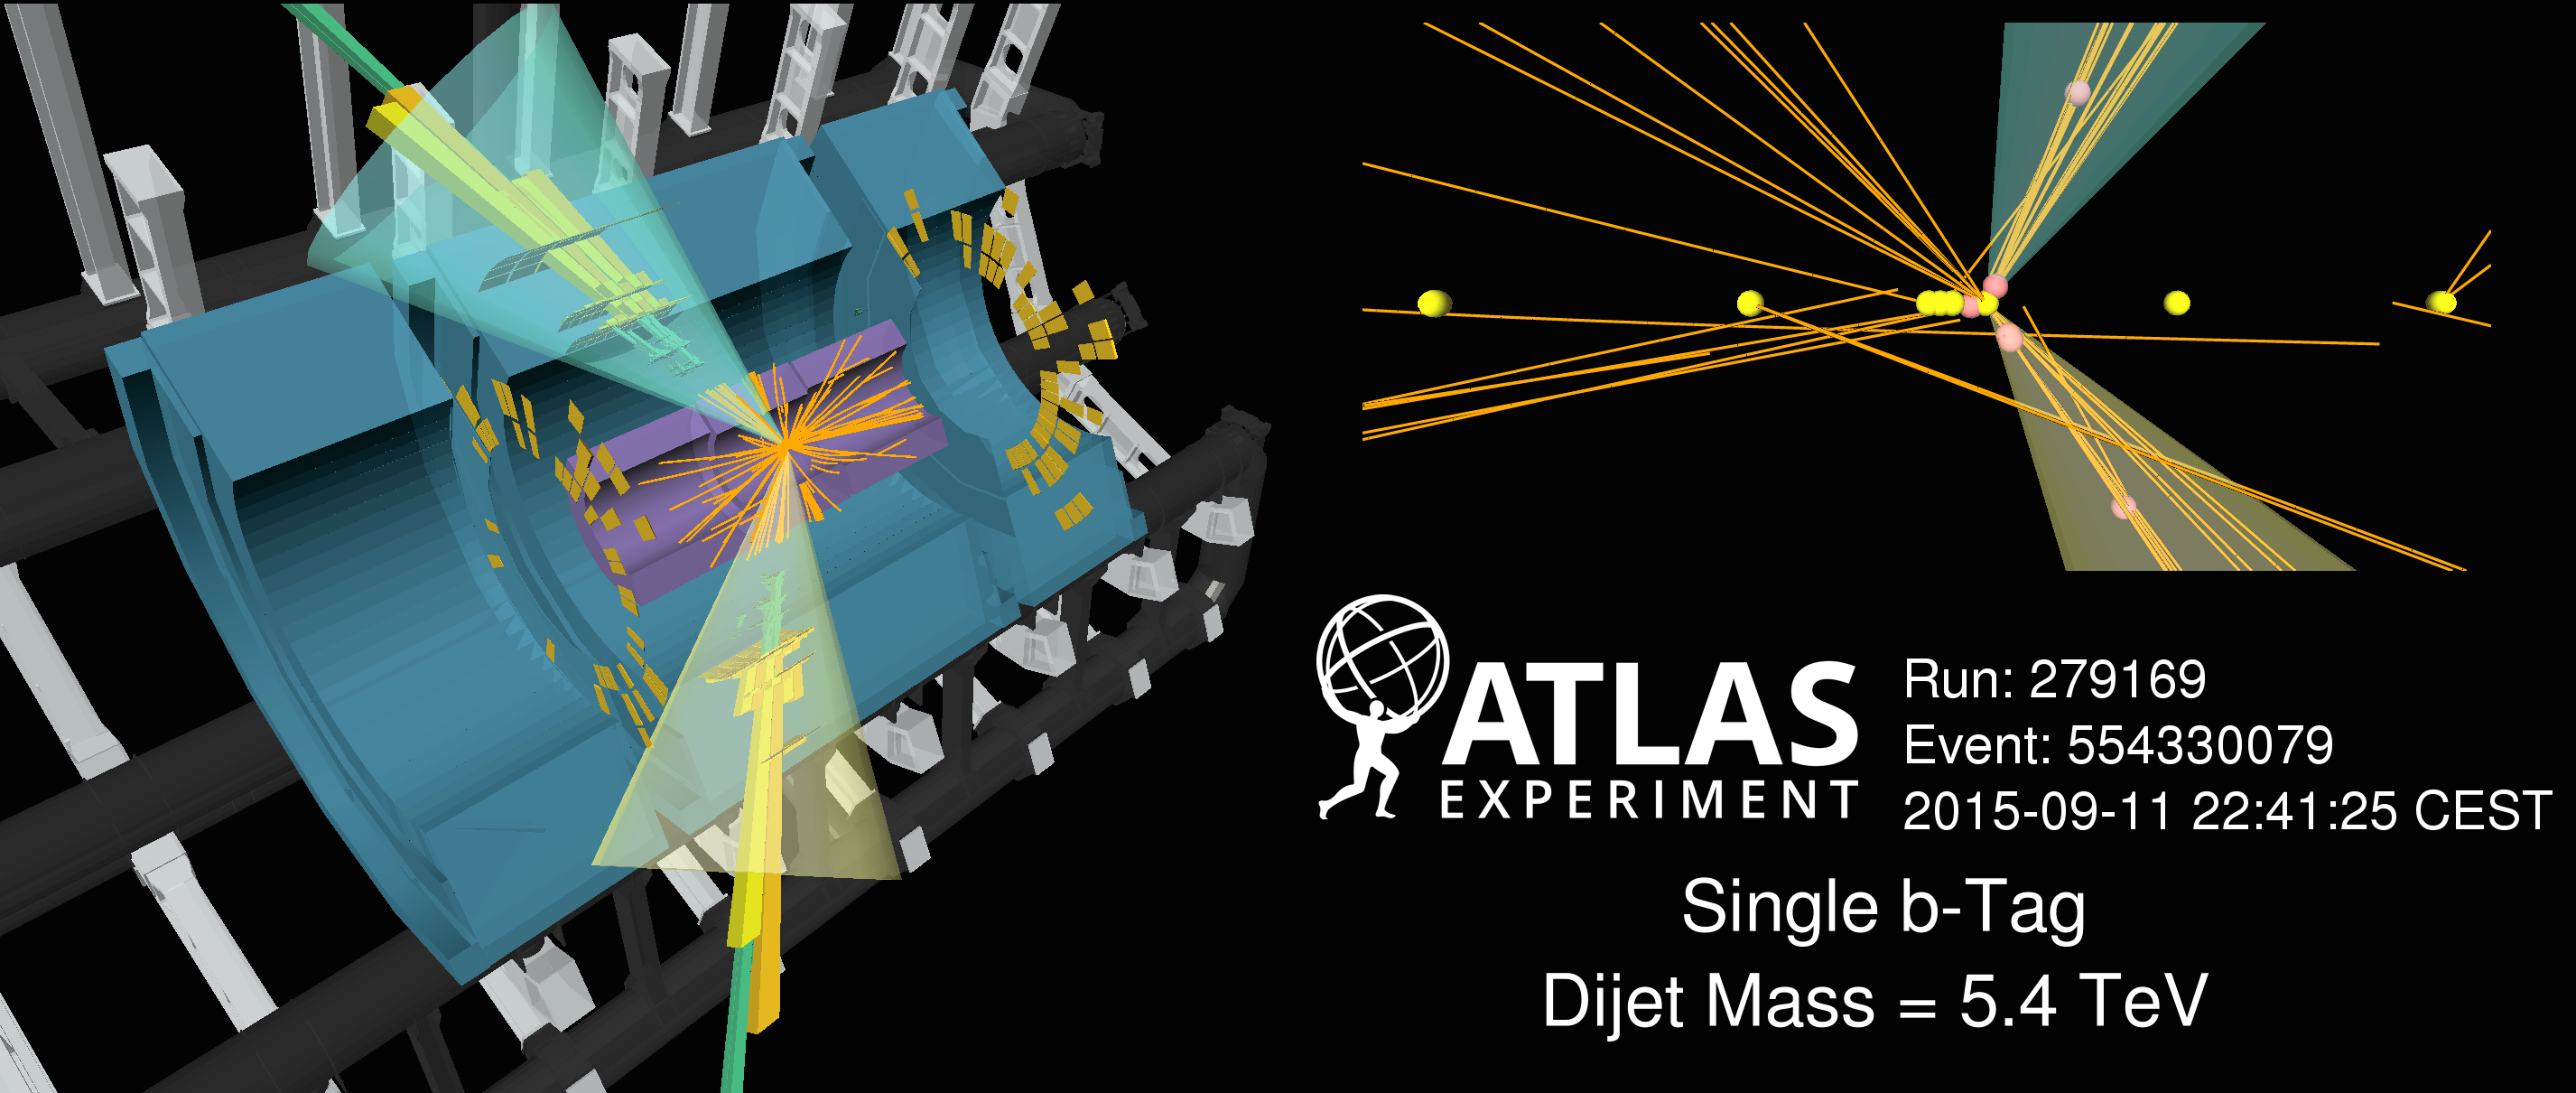
\includegraphics[width=0.95\linewidth, angle=0]{figs/Dibjet/Gen/evt-vp1_b.png}}
  \end{center}
  \caption
      {Event displays showing high~\mjj~events that pass the (a) 2 and (b) $\geq$1 $b$-tag di-$b$-jet event selection.
        The left section of the figures show a cut-away of the ATLAS detector;
        the inner detector is shown in purple, the hadronic calorimeter is shown in blue
        and the toroid magnet and supporting structure is shown in black and grey.
        The upper right section of the figures show a close-up view of the inner tracker in the $r-z$ plane.
        In both sections tracks inside the inner detector are shown in orange
        and energy deposits in the EM and hadronic calorimeter are shown in cyan and yellow respectively.
        The two leading jets formed are indicated by the cones, where a blue cone indicates that the jet has been
        $b$-tagged and a yellow cone shows that it has not.
        The yellow spheres show the primary vertex candidates and the red spheres show the secondary vertex candidates.
      }
  \label{fig:lim-summer_gauss}
\end{figure}

With the event selection now defined
the signal acceptance of the di-$b$-jet analysis is studied
as it helps us understand the performance of the analysis selection
and it will be used as an input to the limit-setting phase of the analysis.
The signal acceptance multiplied by trigger efficiency is defined as the 
the fraction of signal events that would pass the analysis' trigger and event selection.
In addition, as $b$-tagging is a unique cut in our analysis relative to other dijet searches,
we also consider the event-tagging efficiency defined as the fraction of events that pass
$b$-tagging cuts given that the event has passed all other aspects of the event selection.
Signal acceptance and event tagging efficiency are estimated using the
Monte-Carlo signal templates discussed in Section~\ref{sec:evt-s+b}.

For the \verb|Summer16+15| data-set event-selection;
Figure~\ref{fig:evt-ichep_acc}(a) shows the signal acceptance multiplied by trigger efficiency
for the $b^*$ and $Z'$ signal models
as a function of the simulated mass of the signal model
in the case that $b$-tagging is applied and when it is not applied.
Figure~\ref{fig:evt-ichep_acc}(b) shows the event tagging efficiency
for the $b^*$ and $Z'$ for a range of signal mass points
as a function of the reconstructed invariant mass,~\mjj.
In both plots the $b$-tagging category used is labelled in the legend.

There are a few features of the signal acceptance and tagging efficiency that can be commented on.
There is reduced signal acceptance at lower values of simulated mass;
this is because there is a low mass tail of the signal template which lies below the~\mjj~cut
caused by a preference for low values of~\mjj~by the PDFs
\footnote{Parton Distribution Function, see Section~\ref{sec:theo-qcd_pdf}.}.
In addition, the event tagging efficiency decreases at high values of~\mjj;
which is caused by a lower performance of $b$-tagging at high jet-\pT.
\textbf{LM Fix: Discuss high-pT $b$-tagging, in b-tag valid chapter.}.
Finally, we see that the $b^*$ quark has a similar tagging efficiency
as the $Z'$-boson in the $\geq$1 $b$-tag category at high~\mjj;
whilst naively one would expect that the $Z'$-boson should have a higher
event tagging efficiency as it decays to two $b$-quarks,
the gluon from the $b^*$ quark decay can split into a pair of lower~\pT~$b$-quarks
which can often be tagged leading to a similar tagging efficiency.

\begin{figure}[!ht]
  \begin{center}
    \captionsetup[subfigure]{aboveskip=0pt,justification=centering}
    \subcaptionbox{Signal acceptance multiplied \\by trigger efficiency}{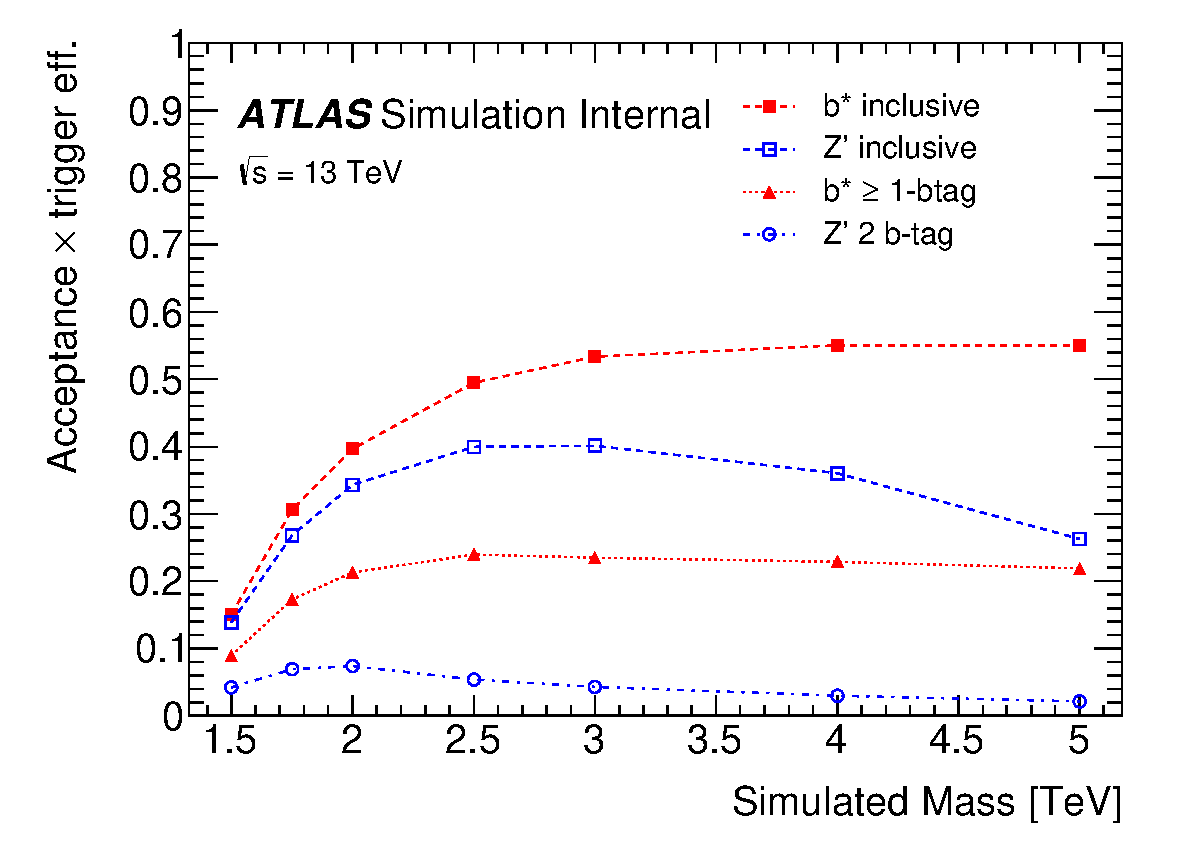
\includegraphics[width=0.48\linewidth, angle=0]{figs/Dibjet/ICHEP/evt-acc.pdf} }
    \subcaptionbox{Event tagging efficiency}{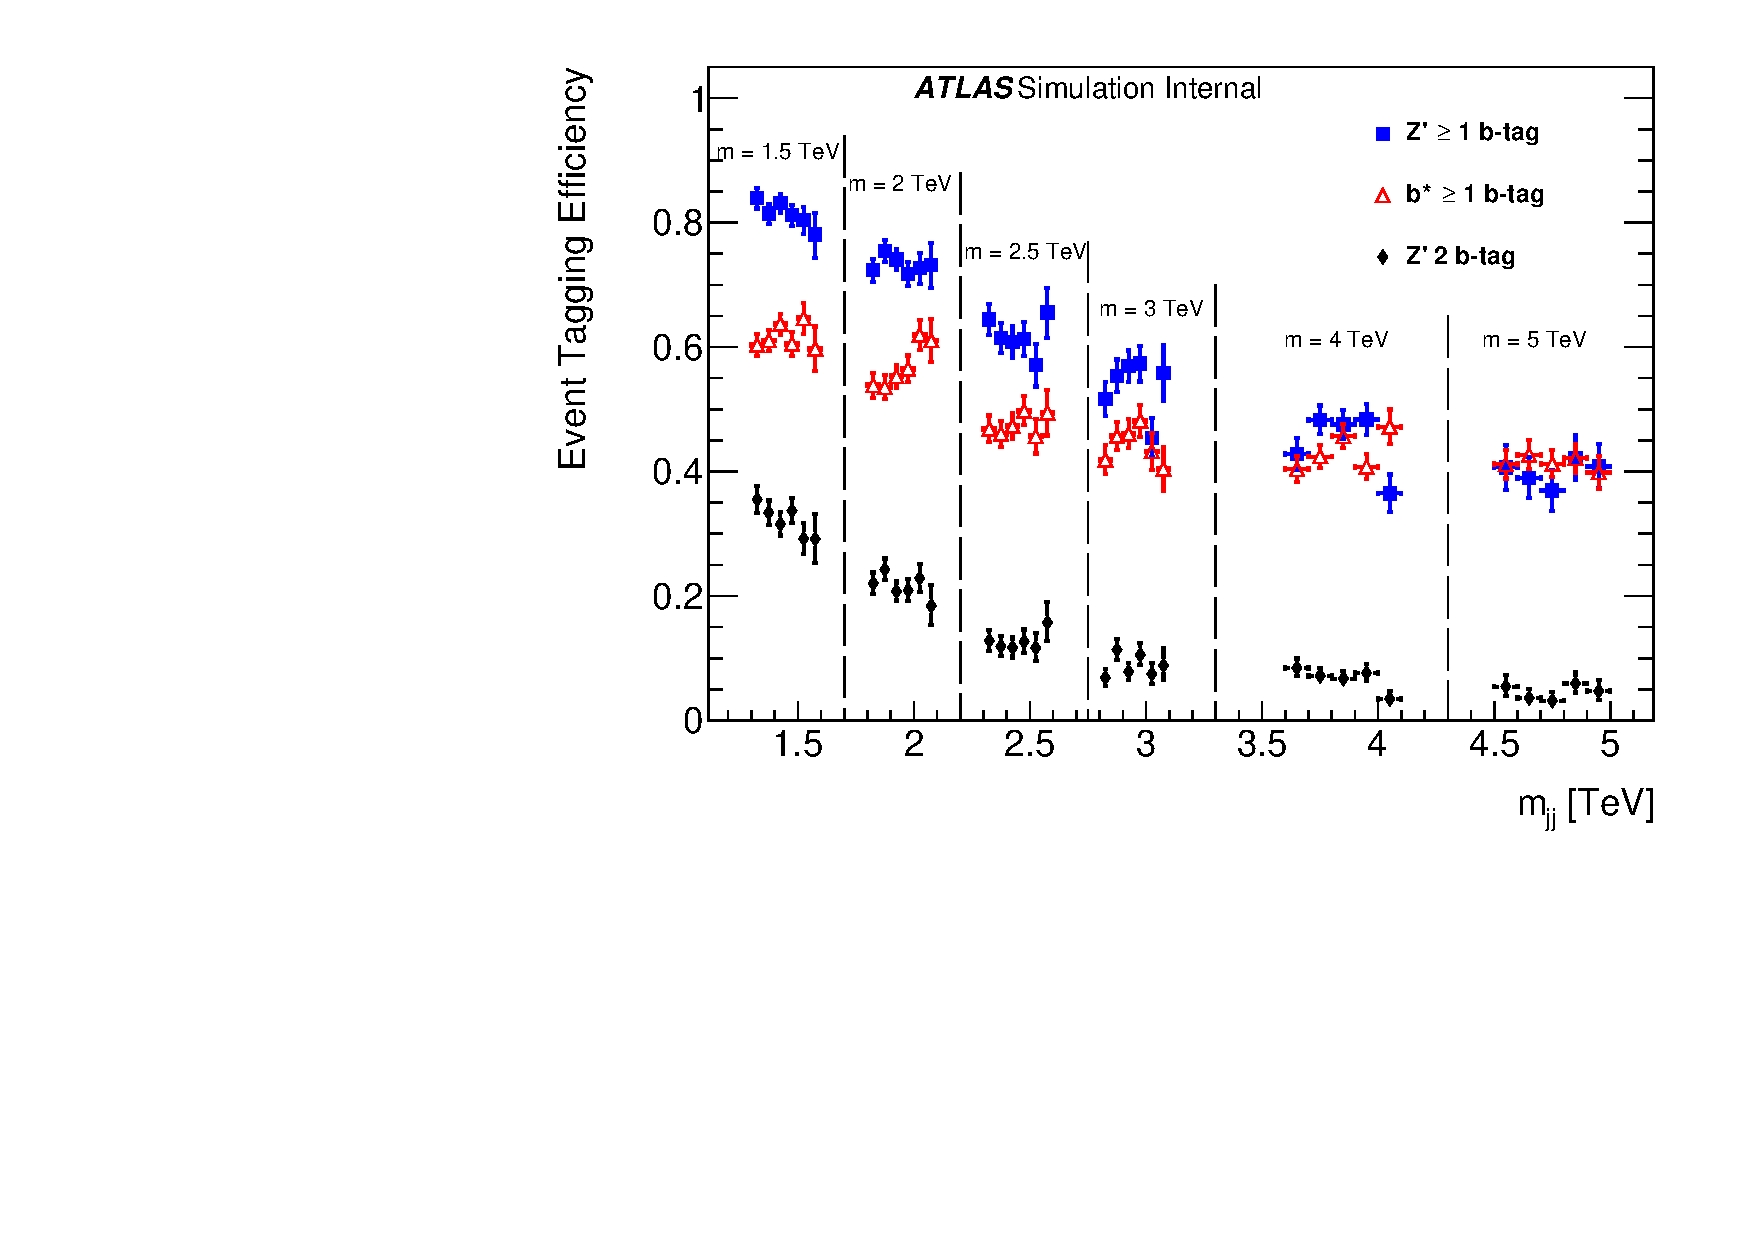
\includegraphics[width=0.48\linewidth, angle=0]{figs/Dibjet/ICHEP/evt-tagEff.pdf} }
  \end{center}
  \caption[Plots to show the acceptance of the \textit{Summer16+15} data-set event selection for the $b^*$ quark and $Z'$-boson signal models.
            Panel (a) shows the signal acceptance multiplied by trigger efficiency as a
            function of the simulated mass of the signal model, in the case where $b$-tagging has been applied and not.
            Panel (b) shows the event tagging efficiency as a function of the reconstructed invariant mass,~\mjj.
            In both figures the $b$-tagging categories used are indicated in the legend.
            Details of the \textit{Summer16+15} data-set event selection are described in the text.]
          {Plots to show the acceptance of the \textit{Summer16+15} data-set event selection for the $b^*$ quark and $Z'$-boson signal models.
            Panel (a) shows the signal acceptance multiplied by trigger efficiency as a
            function of the simulated mass of the signal model, in the case where $b$-tagging has been applied and not.
            Panel (b) shows the event tagging efficiency as a function of the reconstructed invariant mass,~\mjj.
            In both figures the $b$-tagging categories used are indicated in the legend.
            Details of the \textit{Summer16+15} data-set event selection are described in the text.
            Figures taken from~\cite{dibjet-ichep_conf}} 
  \label{fig:evt-ichep_acc}
\end{figure}
